\documentclass[12pt]{article}
\usepackage{geometry}                % See geometry.pdf to learn the layout options. There are lots.
\geometry{letterpaper}                   % ... or a4paper or a5paper or ...
\usepackage{graphicx}
\usepackage{amssymb}
\usepackage{amsthm}
\usepackage{epstopdf}
\usepackage[utf8]{inputenc}
\usepackage[usenames,dvipsnames]{color}
\usepackage[table]{xcolor}
\usepackage{hyperref}

\usepackage{parskip}
\usepackage{enumitem}

\DeclareGraphicsRule{.tif}{png}{.png}{`convert #1 `dirname #1`/`basename #1 .tif`.png}
 
\theoremstyle{definition}
\newtheorem{example}{Example}

\newenvironment{explanation}{%
   \setlength{\parindent}{0pt}
   \itshape
   \color{blue}
}{}

\newenvironment{text}{
}{} 
 
\newcommand{\productname}{Guideo - Audio Guide Platform}
\newcommand{\projectleader}{L. Engleder}
%\newcommand{\documentstatus}{  In process }
\newcommand{\documentstatus}{Submitted}
%\newcommand{\documentstatus}{Released}
\newcommand{\version}{V. 2.01.3}
 
\begin{document}
\begin{titlepage}
\begin{flushright}

\includegraphics[scale=.5]{htlleondinglogo.png}\\
\end{flushright}
 
\vspace{10em}
 
\begin{center}
{\Huge Project Proposal} \\[3em]
{\LARGE \productname} \\[3em]
\end{center}
 
\begin{flushleft}
\begin{tabular}{|l|l|}
\hline
Project Name & \productname \\ \hline
Project Leader & \projectleader \\ \hline
Document state & \documentstatus \\ \hline
Version & \version \\ \hline
\end{tabular}
\end{flushleft}
 
\end{titlepage}
\section*{Revisions}
\begin{tabular}{|l|l|l|}
\hline
\cellcolor[gray]{0.5}\textcolor{white}{Date} & \cellcolor[gray]{0.5}\textcolor{white}{Author} & \cellcolor[gray]{0.5}\textcolor{white}{Change} \\ \hline
September 16, 2019&L. Engleder/P. Quoc/L. Wirth&First version \\ \hline
September 20, 2019&L. Engleder/P. Quoc/L. Wirth& Base information for each section; \\ && proofreading by P. Bauer \\ \hline
September 23, 2019&L. Engleder/P. Quoc/L. Wirth&Minor improvements \\ && and more details;  \\ && proofreading by P. Bauer \\ \hline
September 27, 2019&L. Engleder/P. Quoc/L. Wirth/A. Leeb&writing on planing section \\ \hline
September 29, 2019&L. Engleder/P. Quoc/L. Wirth/A. Leeb&more information in \\ && planning section \\ \hline
September 30, 2019&L. Engleder/P. Quoc/L. Wirth/A. Leeb& improvements on all sections \\ \hline
October 4, 2019&L. Engleder/P. Quoc/L. Wirth/A. Leeb&improvements on all sections\\ \hline
October 7, 2019&L. Engleder/P. Quoc/L. Wirth/A. Leeb&improvements on all sections\\ \hline
October 8, 2019&L. Engleder/P. Quoc/L. Wirth/A. Leeb&graphics and UI description\\ \hline
October 10, 2019&L. Engleder&proof reading and \\ && small adjustments\\ \hline
October 11, 2019&L. Engleder/P. Quoc/L. Wirth/A. Leeb&Milestones\\ \hline
October 13, 2019&L. Wirth&finished Milestones\\ \hline
October 13, 2019&L. Engleder/P. Quoc/L. Wirth/A. Leeb&some changes\\ \hline
October 21, 2019&L. Engleder/P. Quoc/A. Leeb&Initial Situation, Oportunities \\ && and Risks \\ \hline
Ocotber 24, 2019&L. Wirth/L. Engleder&List of Milestones \\ \hline
\end{tabular}
\pagebreak
 
\tableofcontents
\pagebreak
 
\section{Introduction}
\begin{text}
Guideo is a platform for users and creators of audio guides. Depending on the location the user can choose from a diverse catalogue of guides, which in turn deliver an informative and highly enjoyable experience. 
It enables anyone to walk through a city or museum without any prior knowledge of it and learn about a variety of subjects such as culture, history, and art. 
Our app not only offers users a unique way to explore a foreign country, but it also opens doors for anyone who wants to express himself through a highly personal, new kind of creative medium. 
 
\end{text}
\pagebreak
 
\section{Initial Situation}
\begin{text}
Currently, there are some ways for people to get information about their traveling destination.\newline

An established way is to read a physical or online travel guide. Depending on the creator they can be quite interesting and well constructed. Unfortunately they are limited to the constraints of the written word. The recent rise of audio and video platforms has shown that many people consume educational content through these new mediums . Receiving the information in real time also makes the experience of learning more enjoyable. It is also commonly known that there are different types of \href{https://www.tandfonline.com/doi/full/10.1080/0144341042000228834}(learning styles) and that many people learn more effectively through auditory stimulation over reading.\newline
 
Another option for many people is the possibility of hiring a tour guide or joining a bus tour, both promise to offer an educative personalized experience. 
First of all, there is a huge amount of people who are unable to take part in tours because of hearing impairment or slower walking speed.
For people who are travelling alone or with their families these tours can quite expensive as the \href{https://www.guides-in-vienna.at/costs-terms//}{prices} are often fixed.
Since tours are conducted by humans, there are a few limitations by nature. A guide can only handle a certain amount of people per tour, while still having control of the big group. This is especially problematic, when you consider that there are languages which are very sparsely, if at all, supported. \href{https://linz-tours.at}{Linz Tours}, which provide tours in Linz, offer just one guide for Hungarian, Slovakian and Czech. They do not even support a single Asian language. Adding to that, it is possible that tour guides are fully booked, postponed or even cancelled.\newline
 
For many museums, the installment of an audio guide system can be a big financial burden. Especially the purchase of  custom hardware specialized companies seems out of place in our modern connected world. Moreover, a  high number of devices is needed if the museums wants to offer audio guides to everyone. Popular events, like \href{https://www.tips.at/nachrichten/linz/kultur/459167-oberoesterreich-im-kunstfieber-schon-ueber-15-000-besucher-kamen-zu-den-grossen-meistern-in-die-tabakfabrik-linz}{the art exhibition in the Tabakfabrik Linz}, show how museums can be overwhelmed by the high amount of visitors and are therefore not able to provide every visitor with an audio guide.
Additionally, the headsets needs to be cleaned properly at least after one use.
The headsets should not only look good, they also need to be disinfected. Otherwise, \href{https://www.sciencedirect.com/science/article/abs/pii/S019607098580048X}{germs and viruses} stay on the earphones and will infect upcoming users. The most common method to get rid of a fraction of germs and viruses are simply by washing and cleaning the headsets with disinfecting alcohol, but this is not enough. To ensure the highest hygiene level a method called \href{https://www.ncbi.nlm.nih.gov/pmc/articles/PMC6379899/}{Ultraviolet Germicidal Irradiation} (UVGI) is a must. \href{https://pubs.asha.org/doi/abs/10.1044/jshr.1202.326}{UV irradiation} guarantees that nobody will get infected from using borrowed earphones. The problem is that most museums do not have these devices, since they are quite expensive.
But without a regular inspection and cleaning, these systems fail basic hygienic standards and also increase the chance of infecting visitors.
\newline

Although there are audio guides in use in museums there is still no way to enjoy them in a city in general. Our service would provide both locations with fitting guides.

Many guides are prearranged and have a fixed procedure. This grants the follower of the guide little to no flexibility. Even a quick trip to the toilet hinders the guiding group. If the guide is behind time, he will probably stress the people out and even skip some attractions and locations. 
\end{text}
 
\pagebreak
 
\section{General Conditions and Constraints}

\subsection{Framework conditions} 
\begin{text}

We are not planning to spend any money except for the cost of a web hosting server. Additional budget points are possible, but not wanted.\newline

As the app was initially and is still imagined as a mobile app. We would develop the app with Angular, a front-end framework, capable of delivering cross-platform mobile solutions. For the server functionality, we will use NodeJS .\newline
 
At the time of writing, only one of our members gathered experiences with Angular, but we are all familiar with the basics.
We also consider ourselves quite confident in our abilities to learn new skills and technologies.\newline
 
Contacting museums and integrating their audio guides will be a great opportunity to bring quality content onto our platform without the need of extra work. This collaboration is also essential to build a user base and establish ourselves on this market.
It would greatly expand our catalog of guides and help us establish ourselves in the world of museums.\newline
 
There are no commitments as of now. But we are in the process of contacting and talking to museums in our area.

\end{text}

\subsection{Technical conditions}
\begin{text}

We will develop the app with Angular and the server functionality in combination with IntelliJ.

Versioning will be managed over GitHub.\newline
 
There are currently only our 4 Laptops in use and no Server structure available. And 4 android mobile devices for testing.
 
We will use English when documenting and programming.

\end{text}
  
\pagebreak
 
\section{Project Objectives and System Concepts}
 
\subsection{General}
\begin{text}
In general, we aim to create the same experience you could get in museums with their audio guides, but easily accessible through our app. Normally these guides are only available in museums but our routes will be available at iconic sights, in cities, zoos and much more. All of this at fingertips' reach through our mobile application. 

Further on, the museum and zoos in question will easily be able to provide audio guides to their visitors, completely eliminating the need for expensive equipment and maintenance staff.

They only have to provide the audio files and each location on the map or in the building. Our app will recognize if the user is near a placed audio file and play the desired track.

Not only museums or other institutions can create guides, but every one who is willing to create their own experience is welcomed to upload it to our platform for other users to enjoy. These users can then choose between a variety of audio guides covering different topics and presenting the information in various styles.
\end{text}
 
\subsection{Features}
\begin{text}

We will categorise our features into the three main UI views that are visible to the user. More system conditions, technical details will be discussed in the "Details" subsection.

The map view will generally show important locations in your vicinity.
If the user is already listening to a guide he will be shown the best route to get to the locations of the other tracks.\\
Normally there will be only be shown the locations of verified guides like museums and especially high-qualitative user guides.\\
After clicking on a track the user will be shown some general information about the location with the option to rate the individual track. 

In the Explorer View, the user can explore all available audio guides (verified and non-verified) on a map with the respective locations. Alternatively, there will be a list of audio guides structured around locations (e. g. Linz - Linz Kernzone) with essential information such as language, creator, length of time, topics and popularity. Filtering and Sorting will be enabled.

The third main view will inherit the settings, guide creation and the account section. These basic features will not be discussed any further.

\subsubsection{Audio Guide Creation}
Audio guides can be provided by verified users (e. g. museums, cities, etc.) or the community. Users with popularity among the community and a clean record of guides will be given the option to be promoted to verified status

To clarify, a guide is a list of different tracks/files each telling a story or giving information about a certain location/object. If a user decides to create a guide he will be given the option to fully create all of its tracks or to build a compilation out of other guides and his files. A guide should be a creative medium encompassing all the stylistic decisions the guide creator made. \newline

\subsubsection{Geolocation and Tagging System}
When provided and used in a museum the Geo-location based system would be replaced with a tagging system more suited to such an environment.\\
We are planning on offering different options for museums to install their tagging system. The most modern but also most expensive solution would be the installment of beacons that locate users in small spaces and make the experience fluid and easy.\\
Another more simple solution would be to tag the stations or artworks with simple numbers combined with QR-codes which are easily scanned and integrated into the experience.\newline

\subsubsection{Auto-Play and Notifications}
But if a listener encounters a location or object he wants to hear about he will be notified and provided with an explanation of another guide. Still, it will not be played automatically, as we think that if a creator decides not to include a location it was a choice he made out of good reasons.
Out of concern that users could miss important locations or that the amount of points in one guide is low, we will offer a Top Track Mode, which automatically plays the most popular track of a specific location.\newline

A notification will pop up if the user is close to a place or point where a verified audio guide is located, but only if the application is running. A pop-up window will appear if the app runs in the foreground.\\ Otherwise, the notification will show up on the status bar and in the notification inbox. \\
Non-verified audio guides will only be shown in the Explorer View and will not trigger any kind of notification to reduce the chance of annoying the user.\newline

\subsubsection{Rating, Reporting and Verified Status} 
Users that provide audio guides can get verified. Only verified audio guides must be within the regulations and rules. Non-verified audio guides won’t be formally checked but still, need to adhere to the general rules. Users who intentionally provide misinformation, advertise products, etc. will be banned.

To ensure that verified guides are factually correct we will implement a Wikipedia-like system.
All guide content must be verifiable through reliable neutral sources. If reliable sources disagree, then each point of view has to be presented and discussed. 
Anyone can make an annotation to specific timestamps or references of an article. With the agreement of the creator, the change is made permanent.  If a normal user marks a specific fact or statement as wrong, the guide will not fall to unverified status. But if another verified user determines a specific part as inaccurate, the guide will automatically lose its verified status. 
It can regain its status if the guide is edited appropriately.
To simplify the processes of adding references and reviewing articles, guides will have to attach a written script or a small summary of content with concrete facts.

To provide people with recommendations and optimal user experience we plan on collecting some essential data like the languages he or she speaks, preferred language, favorite topics and basic information such as name and email.\newline

\end{text}

\subsection{UI and Design}
\begin{text}
When it comes to User Interface we are thinking of separating the app in three major parts that can be accessed through sliding. 
A map view presents the user with a bird's-eye view of his current location. Depending on the mode and state of the user it shows different kind of things and pinpoints different locations. When a user is already listening to a track he will be shown the other locations and the optimal route of the audio guide. 
If he's just browsing he will be shown the main/start locations of verified guides. Through a toggle on the top right he can choose to view the map in best mode and see the most popular guides to the each of the most important locations.

\begin{figure}[ht]
    \caption{Example of the views of our app}
    \centering
    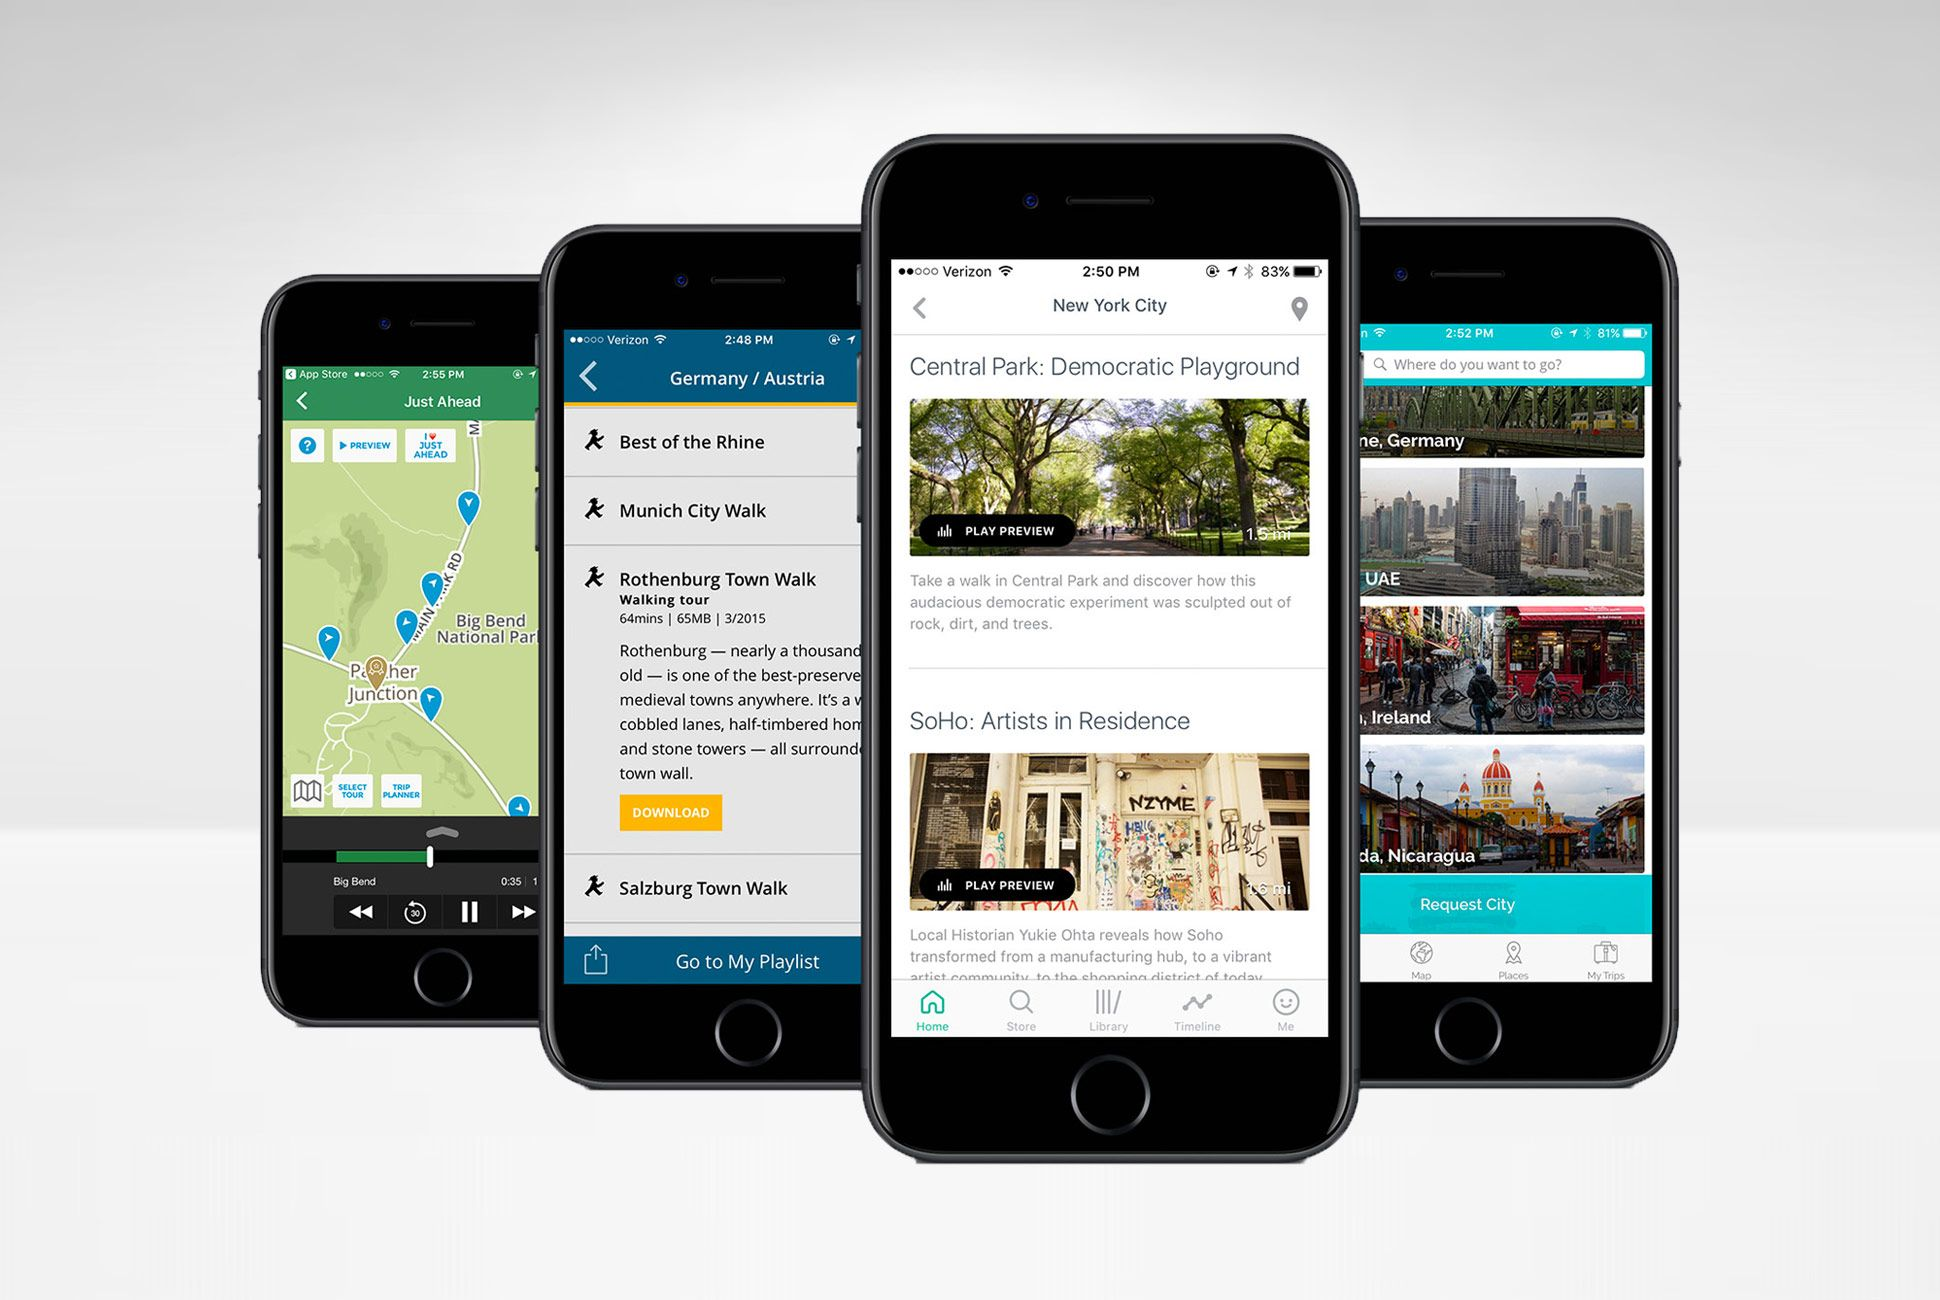
\includegraphics[width=\textwidth]{view_example.jpg}
\end{figure}

Left: Map View with Route Explanation\newline
Middle: Explorer View with Sight on the right
\end{text}

\section{Financial}
\begin{text} 
Our aim is that most of the audio guides are cost-free and that our revenue stems from the purchase of audio guides and advertisements.\newline

To financially sustain ourselves we will use a combination of different sources of revenue. We will employ advertisement on free guides at the beginning and end of the tour. This feature will also push users to buy the ad-free application in exchange for money but, this does not mean that all audio guides (like museums, zoos...) on our platform will be provided for free. \\
When selling the guides we will also take a small commission for our services.\newline

Our platform should also provide a payment system to make the purchase of specific audio guides (museums, zoos...) easy and intuitive. 
\end{text}

\pagebreak
\section{Testing}
\subsection{Ressources}
\begin {text}
At the beginning we get a server from the school for testing purposes.\newline

With our mobile phones the implemented app shall be tested for Android devices. For testing our App on IOS Devices we will ask our classmates.
\end{text}

\subsection{Testing Scenarios}
\begin{text} 
Testing our location-based auto-play will require some testing to ensure that the tracks of each audio guide will be played at the right moment.\newline

We are planning to test the tagging system in our own school as it shares some features as size and basic architectural structure with a normal museum. We will test different methods (QR, Number ...) and try their ease of use.\newline

We would also like to test it at school events like the "Tadeot" to showcase our application and test our system with a bigger user-load.\newline

In order to create an authentic experience we will have to experiment with walking-speeds, radius and other factors that could help the audio guides to flourish.\newline
\end{text}
 
\pagebreak
\section{Opportunities and Risks}

\subsection{Museums, Zoos and Galleries}
\begin{text}
Contacting and collaborating with museums, zoos and art galleries and  is essential to our plan and we are already working on building a relationship with local museums.  Their content and help will establish us as real option for many users.  Moreover, their audio guides are of high quality and would enrich our catalogue in general.
\end{text}

\subsection{Augmented Reality}
\begin{text}
Another opportunity for expanding the app would be to simulate an audio-visual experience through the use of AR-technology. It could be employed in historical settings and sceneries. Although the idea is very interesting it would require far more development time and expertise in the field.\newline
\end{text}

\subsection{Event based Use Cases}

\subsubsection{Working with Photo or Art Galleries}
\begin{text}
We would like to collaborate with the Kunstuniversität Linz and their students gallery called "Galerie WHA". The creators of each piece would write a small segment about their work and we would integrate each part into a big audio guide of the gallery. This enables visitors to experience the art, while learning about the artist's thought process. Updating and substituting could easily be managed through our platform.
\end{text}

\subsubsection{HTL Leonding's Photo contest}
\begin{text}
The same principle as in "galerie WHA" could be applied to our own school's photo contest. It is one of the biggest events every year and we would like to make it even bigger.  With our system the contest is not only about individual pictures, but also about telling a compelling story. Technical details can also easily be conveyed to the visitors. Our app would definitely make the experience more immersive and well-rounded.
\end{text}

\subsubsection{Tadeot at Schools (Day of open Doors)}
\begin{text}
Every year hundreds of young middle school pupils visit our school to make themselves a picture of the HTL Leonding. Normally, some of our own students are selected to accompany the children and their parents through the building, while sharing important information about each subject and room. We would employ our guides to relieve the students and offer the option of using an audio guide. 
It will also be a great opportunity to test our tagging system with a considerate amount of users.
\end{text}

\subsection{Guide Creation}
\begin{text}
Through releasing guides we, our-selves, created, we hope to boost our in-app activity and make our product more presentable in the early stages. It enables us to let other people test and try out the first guides.\newline

We would also document our process and create a tutorial to simplify the process for creators, who are interested in developing guides. \newline
\end{text}

\subsection{Use of Beacons}
\begin{text}
 The use of beacons like Estimote's \href{https://estimote.com/}{Beacon} offers the opportunity of creating an even more smooth and seamless experience. The are already used in a small hand of museums. It really is an exciting technology with great potential for our project. Offering support for these systems and enabling museums to install them could really extend our current understanding of audio guides. 
 
\end{text}

\subsection{Risks}
\begin{text}
We could face the risk that our catalogue is too small to consider it as an option. The only real solution for this problem would be to advertise our app and encourage the creative minds of other platforms to join.  This is not our first option as it is financially draining and requires a lot of knowledge and effort in marketing and advertising. This risk goes hand in hand with our second concern.

One of the biggest risks would just be the absence of any traction and popularity among Museums, Zoos and the like. They are our primary means to generate a user base and attract creators to our platform. Other ways demand far more resources and time to be successful. 
Without content from the museum, the creation of extra content would also need to be arranged.
\end{text}

\section{Planning}
\subsection{Milestones}
\begin{tabular}{| m{9em} | m{9cm} | m{4cm} |}
    \cellcolor[gray]{0.5}\textcolor{white}{Milestone} &
    \cellcolor[gray]{0.5}\textcolor{white}{Definition of Done} &
    \cellcolor[gray]{0.5}\textcolor{white}{Date} \\ \hline
    
    Database structure and fundamental server functionality & 
    \begin{itemize} [topsep=0.2cm]
        \item Creating a database in hold of account data, guide information(name, description) and geofences
    \end{itemize} \nointerlineskip &
    30th November 2019 \\ \hline
    
    Account and Management &
    \begin{itemize} [topsep=0.2cm]
        \item creating login view in App
        \item create account management system
    \end{itemize} \nointerlineskip &
    10th December 2019 \\ \hline
    
    Audio Guide Streaming &
    \begin{itemize}
        \item UI Support for basic functions
        \item automatic playing + consistent stream
    \end{itemize} \nointerlineskip &
    20th December 2020 \\ \hline
    
    Networking and Contacting Collaborators &
    \begin{itemize} [topsep=0.2cm]
        \item Contacting 15 local museums through email
        \item Talking about the sale of guides
        		  \item Contacting specific events
    \end{itemize} \nointerlineskip &
    20th December 2019\\ \hline
    
    Geolocation, \linebreak Geofences, \linebreak Notifications &
    \begin{itemize} [topsep=0.2cm]
        \item Geofence initialization and management
        \item Notifications and toggle switch
        \item Geofences in stand-by mode     
    \end{itemize} \nointerlineskip &
     20th February 2019  \\ \hline
    
    Tagging System &
    \begin{itemize} [topsep=0.2cm]
        \item Number Tagging
        \item QR-Code scanning + Selection
    \end{itemize} \nointerlineskip &
    30th March 2020 \\ \hline
     
    Route Finding and Explorer View &
    \begin{itemize} [topsep=0.2cm]
        \item GMaps API integration
        \item Best Mode
        \item Other Routes and Support for other means of Transportation (Car, Bike ...)
    \end{itemize} \nointerlineskip &
    30th April 2020 \\ \hline
    
    Payment System &
    \begin{itemize} [topsep=0.2cm]
        \item Incorporating Payment System into app
        \item Museum Price Settings
    \end{itemize} \nointerlineskip &
    20th May 2020 \\ \hline
    
    Guide Creation System (Recording and Tagging) &
    \begin{itemize} [topsep=0.2cm]
        \item file uploading and management
        \item database integration
        \item location - track mapping
        \item geofence settings + best route
    \end{itemize} \nointerlineskip &
    30th June 2020 \\ \hline
    
    Archive + Rating + Reporting &
    \begin{itemize} [topsep=0.2cm]
        \item Implementing System for Fact-Checking
    	\item User Interaction (Comments, Rating, Report)
        \item Archive Feature on Webpage
    \end{itemize} \nointerlineskip &
    30th November 2020 \\ \hline
\end{tabular}

\subsection{Members}
\begin{tabular}{|l|l|}
\hline
\cellcolor[gray]{0.5}\textcolor{white}{Name} & \cellcolor[gray]{0.5}\textcolor{white}{Role}\\ \hline
Lucas Engleder & Project Leader, Mobile Co-Master and Database Assistant\\ \hline
Patrick Quoc & Mobile Master\\ \hline
Lukas Wirth & Seamodea \\  \hline
Alexander Leeb & Database Master and Server Assistant \\ \hline
\end{tabular}

Role Explanation:
\begin{itemize}
    \item Seamodea
    \begin{itemize}
        \item \textbf{Se}rver
        \item \textbf{A}nd
        \item \textbf{Mo}bile \textbf{De}sign
        \item \textbf{A}rchitect
    \end{itemize} 
\end{itemize}
\subsection{Resources}
\subsubsection{Human Resources}
\begin{text}
Our project is actually a school project which disables us to really consider external programming help, outside of our core team members. We wouldn't use this option anyway as we see this project not only as necessary work, but as an opportunity to learn new things and try innovative technologies.

But regarding design, we are bearing in mind that our capabilities might be limited and in need of an overlooking eye. Possible candidates are colleagues in our school's design branch.\end{text}

\subsubsection{Licenses and Server}
\begin{itemize}
\item License for Jetbrains' IntelliJ Ultimate Edition IDEA to develop Angular Apps.
\item Microsoft's Visual Studio Code and Drifty Co.'s Ionic are under the MIT License.
\item Database License
\end{itemize}

We are considering buying a server if our school isn't able to provide one. In the case of a possible purchase we would need a server with storage capabilities to accommodate our file space needs.

\subsection{Project Management}
\begin{itemize}
    \item Start of project: 14th or 18th October 2019
    \item End of project: End of 5th grade
    \item First Prototype available: 29th February 2020 (First day of school after semester vacation)
    \item Begin of implementation work: 18th October 2019
    \item Big blocks of work
    \begin{itemize}
        \item Database and Server Structure
        \item Localization and Notifications
        \item Audio Guide Streaming
        \item Account Login, Authentication and Management
        \item Route Finding and Google maps integration in general
    \end{itemize}
    \item With enough dedication and without major problems in development we estimate it to be hard but quite possible
    \item As already mentioned we will need a server for our application.
    
\end{itemize} 

\pagebreak
\section{Sources}
\begin{text}
 [1] https://www.tandfonline.com/doi/full/10.1080/0144341042000228834\\
 [2] https://www.guides-in-vienna.at/costs-terms//\\
 [3] https://linz-tours.at\\
 [4] https://www.tips.at/nachrichten/linz/kultur/459167-oberoesterreich-im-kunstfieber-schon-ueber-15-000-besucher-kamen-zu-den-grossen-meistern-in-die-tabakfabrik-linz\\
 [5] https://www.sciencedirect.com/science/article/abs/pii/S019607098580048X\\
 [6] https://www.ncbi.nlm.nih.gov/pmc/articles/PMC6379899/\\
 [7] https://pubs.asha.org/doi/abs/10.1044/jshr.1202.326\\
\end{text}
\end{document} 
